\section{Filtering}
Filtering of raw point clouds is required because of several different reasons. The number of points delivered to the modelling component from the raw point clouds is huge, so filtering non-interesting points away creating a region-of-interest (ROI) in the raw point clouds. Lowering the number points in each cloud delivered to the modelling component is required such the workload can be kept within an acceptable range. The number of points can be further reduced by down-sampling the points left in the ROI by the cut-off filter. A voxel-grid filter utilised for down-sampling also creates the advantage of equal sampling density, but the disadvantage is that the down-sampling means loss of information, and therefore there is a trade off between speed and level of detail of the reconstruction process.  

\begin{figure}[htb]
	\begin{center}
		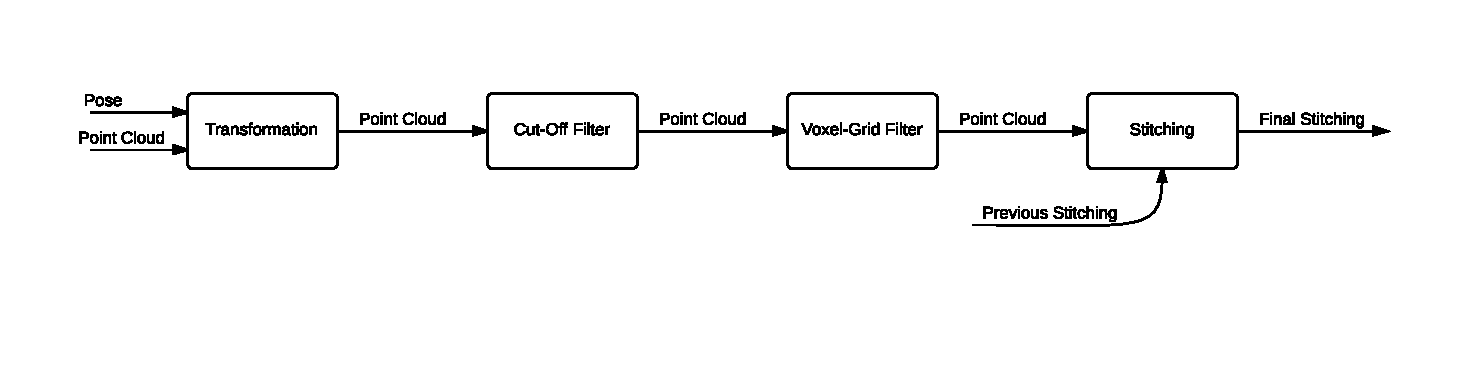
\includegraphics[scale=0.6,trim=20 70 0 20]{graphics/07_modelling/FilterFlow.pdf}%trim=l b r t
		\caption{Illustrates the flow through the filter.}
		\label{fig:filter_flow}
	\end{center}
\end{figure}

In figure \ref{fig:filter_flow} an illustration of the flow through the filter can be seen. The vision layer is delivering a point cloud for each individual view, along with this point cloud a pose of the frame in which the points are recorded is delivered. These two sets of data is delivered to the ROS node which handles filtering, this node filters each individual cloud and stitches each of them together in a common cloud. This common cloud, when finished, is sent to the reconstruction layer. In the sections below is a brief description of the components shown in figure \ref{fig:filter_flow}. 

\subsection{Point cloud library}
The Point Cloud Library (PCL) utilised in this project is a library which provide functionality for working on 3D point clouds. PCL delivers a variety of functionality such as filters, segmentation, surface reconstruction, kd- and oc-trees, visualisation, etc. PCL can be found at http://www.pointclouds.org/, along with documentation and tutorials.

\subsection{Point cloud transformation}
Messages received from the vision layer needs to be processed before filtering. This is because the messages delivered to the modelling component contain a point cloud and a pose of the current camera view. The coordinates of the individual points in the cloud are related to the camera frame, but this frame is moving around the object so a transformation of points is needed such they can be related a common static frame.

\begin{figure}[htb]
	\begin{center}
		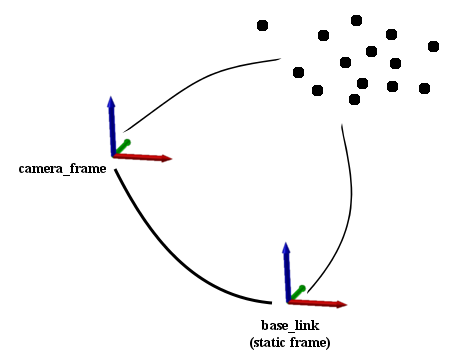
\includegraphics[scale=0.7,trim=0 0 0 0]{graphics/07_modelling/pctransform.png}%trim=l b r t
		\caption{Illustrates points in different frames.}
		\label{fig:filtering_transform}
	\end{center}
\end{figure}

\subsection{Cut-off filter}
The cut-off filter utilised is the implementation from PCL, \texttt{pcl::PassThrough< \ldots >}. A cut-off filter is utilised to create a ROI in the transformed point cloud, partly because the number of points needs to be reduced with respect to processing time and then because the region in which the object resides is fairly small to the region which is recorded by the camera.

\subsection{Voxel-grid filter}
The voxel-grid down-samples the left overs from the cut-off filtering. The down-sampling causes loss of information which mean that surface details are lost in the process, so the amount of down-sampling should be chosen with respect to processing time versus level of detail to be reconstructed. The PCL library luckily have such functionality (\texttt{pcl::VoxelGrid< \ldots >}) which is utilised in the filtering sub-component.\\
\\
The voxel-grid filter works by splitting down the ROI into smaller regions (voxels) of certain resolution in which each of the voxels are analysed. Figure \ref{fig:filtering_voxel_grid} show the principle of the voxel-grid. A new point is approximated for each voxel, the new point is approximated by the points centroid which is contained in the voxel. This method is a little slower compared to just placing the new point in the center of the voxel, but it helps save some more detailed information about the surface curvature.
\begin{figure}[htb]
	\begin{center}
		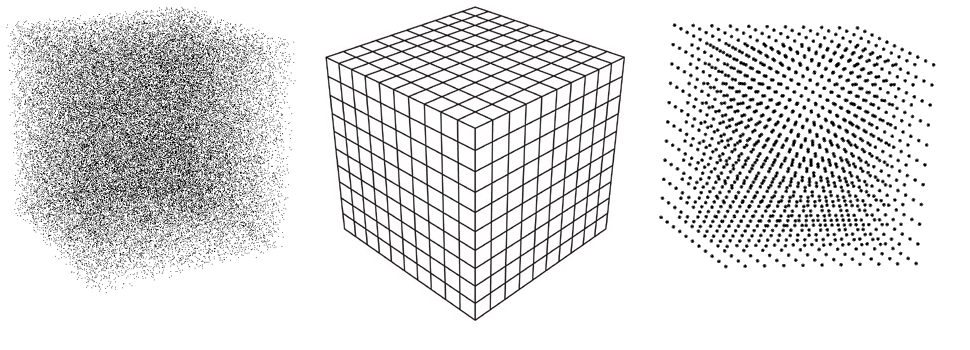
\includegraphics[scale=0.4,trim=0 0 0 0]{graphics/07_modelling/voxelgrid.png}%trim=l b r t
		\caption{Illustrates the down sampling principle of the voxel-grid filter. The left point cloud is down sampled through a set of virtual cubes, which leaves the right cloud after processing the input. A uniform distribution of points is obtained this way for instance.}
		\label{fig:filtering_voxel_grid}
	\end{center}
\end{figure}

\subsection{Point cloud stitching}
\marginnote{Subsection not finished}

The individual point clouds from the individual views of the object are passed through the filter, the individual cloud is then stitched into another common cloud which is assembled from a number of individual clouds, predetermined by the decision making layer. The stitching of each cloud happens in the static frame, due to the transformation of the input to the filter node. The point clouds are stitched in the order at which they are received, thus the first frame becomes a sort of reference frame for the following frames. This is because the algorithm used for stitching the clouds together actually calculates a transform at which new incoming point clouds are transformed. The algorithm utilised for stitching is Iterative Closest Point (ICP). This is also implemented in in PCL and therefore this implementation (\texttt{pcl::IterativeClosestPointNonLinear< \ldots , \ldots >}) of the algorithm utilised. The ICP algorithm has it downsides. For example if a cloud is not aligned correctly, this will cause an error to propagate thought to the following clouds which could lead to a rather distorted model of the object of interest\cite{choe2007registration}. The algorithm will be described in further details in chapter \texttt{ref??}\marginnote{Ref til calibration chapter}.

\subsection{Results}
Preliminary results of the point cloud stitching is shortly presented and discussed here. 

\begin{figure}[htb]
	\begin{center}
		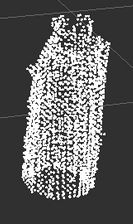
\includegraphics[scale=0.7,trim=0 0 0 0]{graphics/07_modelling/bottle.png}%trim=l b r t
		\caption{Illustrates a stitching of a water bottle. (Carmine data).}
		\label{fig:bottle}
	\end{center}
\end{figure}

\noindent As seen in figure \ref{fig:bottle} the stitching seems reasonable compared to figure \texttt{Bottle figure} \marginnote{Picture of bottle needed}. Inspecting the stitching further reveals a layered structure due to bad alignment as seen in figure \ref{fig:bottle_slice}.

\begin{figure}[htb]
	\begin{center}
		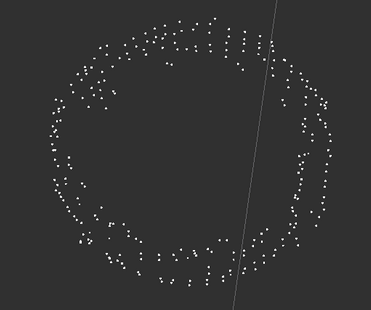
\includegraphics[scale=0.7,trim=0 0 0 0]{graphics/07_modelling/slice.png}%trim=l b r t
		\caption{Illustrates a slice of the stitching seen in figure \ref{fig:bottle}. (Carmine data).}
		\label{fig:bottle_slice}
	\end{center}
\end{figure}

\noindent The slice of the stitching seen in figure \ref{fig:bottle_slice} indicates that the alignment of the individual point clouds are not perfect. This can be causes by the measurements not being perfect due to uncertainties in the system. It is suggested that measuring uncertainties and non-calibrated frames is creating the effect seen in slice of the bottle.\\
\\
It is not known if the reconstruction scheme can handle this layering in the point cloud, but it is assumed it can, but testing this will reveal if the reconstruction method is capable of reconstructing an approximation of the surface of an object.